% 注意事项:编译两次,以确保目录、页码完整显示

\def\allfiles{}

\documentclass[14pt,a4paper,UTF8,twoside]{article}

% Formatting Packages ——————————————————————————————————————
\usepackage{multicol}
\usepackage{multirow}
\usepackage{enumitem}
\usepackage{indentfirst}
\usepackage[toc]{multitoc}

% Math & Physics Packages ————————————————————————————
\usepackage{amsmath, amsthm, amsfonts, amssymb}
\usepackage{setspace}
\usepackage{physics}
\usepackage{cancel}
\usepackage{nicefrac}
\usepackage{unicode-math} % 允许数学公式使用特定字体

% Image-related Packages —————————————————————————————
\usepackage{float} % 浮动体环境
\usepackage{subcaption} % 子图包
\usepackage{graphics, graphicx}
\usepackage{tikz, tikz-qtree}
\usetikzlibrary{arrows.meta}
\usepackage{pgfplots}
\pgfplotsset{compat=1.18}
\usepackage{xcolor}
\usepackage{fourier-orns}
\usepackage{lipsum}

% Colour Palette ——————————————————————————————————————
\definecolor{merah}{HTML}{F4564E}
\definecolor{merahtua}{HTML}{89313E}
\definecolor{biru}{HTML}{60BBE5}
\definecolor{birutua}{HTML}{412F66}
\definecolor{hijau}{HTML}{59CC78}
\definecolor{hijautua}{HTML}{366D5B}
\definecolor{kuning}{HTML}{FFD56B}
\definecolor{jingga}{HTML}{FBA15F}
\definecolor{ungu}{HTML}{8C5FBF}
\definecolor{lavender}{HTML}{CBA5E8}
\definecolor{merjamb}{HTML}{FFB6E0}
\definecolor{mygray}{HTML}{E6E6E6}
\definecolor{mygreen}{rgb}{0,0.6,0}
\definecolor{mymauve}{rgb}{0.58,0,0.82}

% Theorems ————————————————————————————————————————————
\usepackage{tcolorbox}
\usepackage{changepage}
\tcbuselibrary{skins,breakable,theorems}

\newcounter{hitung}
\setcounter{hitung}{\thesection}

\makeatletter
	% Proof 证明如下
	\def\tcb@theo@widetitle#1#2#3{\hbox to \textwidth{\textsc{\large#1}\normalsize\space#3\hfil(#2)}}
	\tcbset{
		theorem style/theorem wide name and number/.code={ \let\tcb@theo@title=\tcb@theo@widetitle},
		proofbox/.style={skin=enhancedmiddle,breakable,parbox=false,boxrule=0mm,
			check odd page, toggle left and right, colframe=black!20!white!92!hijau,
			leftrule=8pt, rightrule=0mm, boxsep=0mm,arc=0mm, outer arc=0mm,
			left=3mm,right=3mm,top=0mm,bottom=0mm, toptitle=0mm,
			bottomtitle=0mm,colback=gray!3!white!98!biru, before skip=8pt, after skip=8pt,
			before={\par\vskip-2pt},after={\par\smallbreak},
		},
	}
	\newtcolorbox{ProofBox}{proofbox}
	\makeatother
	
	\let\realproof\proof
	\let\realendproof\endproof
	\renewenvironment{proof}[1][Prove:]{\ProofBox\strut\textsc{#1}\space}{\endProofBox}
        \AtEndEnvironment{proof}{\null\hfill$\blacksquare$}
        % Definition 定义环境
	\newtcbtheorem[use counter=hitung, number within=section]{dfn}{定义}
	{theorem style=theorem wide name and number,breakable,enhanced,arc=3.5mm,outer arc=3.5mm,
		boxrule=0pt,toprule=1pt,leftrule=0pt,bottomrule=1pt, rightrule=0pt,left=0.2cm,right=0.2cm,
		titlerule=0.5em,toptitle=0.1cm,bottomtitle=-0.1cm,top=0.2cm,
		colframe=white!10!biru,
		colback=white!90!biru,
		coltitle=white,
		shadow={1.3mm}{-1.3mm}{0mm}{gray!50!white}, % 添加阴影
        coltext=birutua!60!gray, title style={white!10!biru}, rbefoe skip=8pt, after skip=8pt,
		fonttitle=\bfseries,fontupper=\normalsize}{dfn}

	% 答题卡
	\newtcbtheorem[use counter=hitung, number within=section]{ans}{解答}
	{theorem style=theorem wide name and number,breakable,enhanced,arc=3.5mm,outer arc=3.5mm,
		boxrule=0pt,toprule=1pt,leftrule=0pt,bottomrule=1pt, rightrule=0pt,left=0.2cm,right=0.2cm,
		titlerule=0.5em,toptitle=0.1cm,bottomtitle=-0.1cm,top=0.2cm,
		colframe=white!10!biru,
		colback=white!90!biru,
		coltitle=white,
		shadow={1.3mm}{-1.3mm}{0mm}{gray!50!white}, % 添加阴影
        coltext=birutua!60!gray, title style={white!10!biru}, before skip=8pt, after skip=8pt,
		fonttitle=\bfseries,fontupper=\normalsize}{ans}

	% Axiom
	\newtcbtheorem[use counter=hitung, number within=section]{axm}{公理}
	{theorem style=theorem wide name and number,breakable,enhanced,arc=3.5mm,outer arc=3.5mm,
		boxrule=0pt,toprule=1pt,leftrule=0pt,bottomrule=1pt, rightrule=0pt,left=0.2cm,right=0.2cm,
		titlerule=0.5em,toptitle=0.1cm,bottomtitle=-0.1cm,top=0.2cm,
		colframe=white!10!biru,colback=white!90!biru,coltitle=white,
		shadow={1.3mm}{-1.3mm}{0mm}{gray!50!white!90}, % 添加阴影
        coltext=birutua!60!gray,title style={white!10!biru},before skip=8pt, after skip=8pt,
		fonttitle=\bfseries,fontupper=\normalsize}{axm}
 
	% Theorem
	\newtcbtheorem[use counter=hitung, number within=section]{thm}{定理}
	{theorem style=theorem wide name and number,breakable,enhanced,arc=3.5mm,outer arc=3.5mm,
		boxrule=0pt,toprule=1pt,leftrule=0pt,bottomrule=1pt, rightrule=0pt,left=0.2cm,right=0.2cm,
		titlerule=0.5em,toptitle=0.1cm,bottomtitle=-0.1cm,top=0.2cm,
		colframe=white!10!merah,colback=white!75!pink,coltitle=white, coltext=merahtua!80!merah,
		shadow={1.3mm}{-1.3mm}{0mm}{gray!50!white!90}, % 添加阴影
		title style={white!10!merah}, before skip=8pt, after skip=8pt,
		fonttitle=\bfseries,fontupper=\normalsize}{thm}
	
	% Proposition
	\newtcbtheorem[use counter=hitung, number within=section]{prp}{命题}
	{theorem style=theorem wide name and number,breakable,enhanced,arc=3.5mm,outer arc=3.5mm,
		boxrule=0pt,toprule=1pt,leftrule=0pt,bottomrule=1pt, rightrule=0pt,left=0.2cm,right=0.2cm,
		titlerule=0.5em,toptitle=0.1cm,bottomtitle=-0.1cm,top=0.2cm,
		colframe=white!10!hijau,colback=white!90!hijau,coltitle=white, coltext=hijautua!80!brown,
		shadow={1.3mm}{-1.3mm}{0mm}{gray!50!white}, % 添加阴影
		title style={white!10!hijau}, before skip=8pt, after skip=8pt,
		fonttitle=\bfseries,fontupper=\normalsize}{prp}


	% Example
	\newtcolorbox[use counter=hitung, number within=section]{cth}[1][]{breakable,
		colframe=white!10!jingga, coltitle=white!90!jingga, colback=white!85!jingga, coltext=black!10!brown!50!jingga, colbacktitle=white!10!jingga, enhanced, fonttitle=\bfseries,fontupper=\normalsize, attach boxed title to top left={yshift=-2mm}, before skip=8pt, after skip=8pt,
		title=Contoh~\thetcbcounter \ \ #1}

	% Catatan/Note
	\newtcolorbox{ctt}[1][]{enhanced, 
		left=4.1mm, borderline west={8pt}{0pt}{white!10!kuning}, 
		before skip=6pt, after skip=6pt, 
		colback=white!85!kuning, colframe= white!85!kuning, coltitle=orange!60!kuning!25!brown, coltext=orange!60!kuning!25!brown,
		fonttitle=\bfseries,fontupper=\normalsize, before skip=8pt, after skip=8pt,
		title=\underline{Catatan}  #1}
	
	% Komentar/Remark
	\newtcolorbox{rmr}[1][]{
		,arc=0mm,outer arc=0mm,
		boxrule=0pt,toprule=1pt,leftrule=0pt,bottomrule=5pt, rightrule=0pt,left=0.2cm,right=0.2cm,
		titlerule=0.5em,toptitle=0.1cm,bottomtitle=-0.1cm,top=0.2cm,
		colframe=white!10!kuning,colback=white!85!kuning,coltitle=white, coltext=orange!60!kuning,
		fonttitle=\bfseries,fontupper=\normalsize, before skip=8pt, after skip=8pt,
		title=Komentar  #1}

\usepackage{booktabs} % 表格库
\usepackage{titlesec} % 标题库
\usepackage{fancyhdr} % 页眉页脚库
\usepackage[sorting=none]{biblatex}
\usepackage{array}
\addbibresource{references.bib} % 指定你的.bib文件名称

\date{} % 留空,以让编译时去除日期

%———————————————注意事项—————————————————%

% 1、如果编译显示失败,但没有错误信息,就是 filename.pdf 正在被占用
% 2、在文件夹中的终端使用 Windows > xelatex filename.tex 也可编译

%—————————————华东师范大学———————————————%

% 论文制作时须加页眉,页眉从中文摘要开始至论文末
% 偶数页码内容为:华东师范大学硕士学位论文,奇数页码内容为学位论文题目

%————————定义 \section 的标题样式————————%

% 注意:\chapter 等命令,内部使用的是 \thispagestyle{plain} 的排版格式
% 若需要自己加上页眉,实际是在用 \thispagestyle{fancy} 的排版格式
% 加上下面这一段指令,就能够让 \section 也使用 fancy 的排版格式
% 本质就是让目录、第一页也能够显示页眉、页脚

\fancypagestyle{plain}{
  \pagestyle{fancy}
}

\title{华东师范大学软件学院实验报告} % 模板
\titleformat{\section}
    {\normalfont\bfseries\Large} % 字体大小、字体系列(\bfseries 为加粗)
    {\thesection}{1em}{}

% ———————————设置章节的中文格式———————————%
\renewcommand\thesection{\chinese{section} \hspace{0pt}}
\renewcommand\thesubsection{\arabic{subsection} \hspace{0pt}}
% \renewcommand\thesubsubsection{\alph{subsubsection} \hspace{0pt}} % 字母编号
% \hspace{0pt} 是为了确保在章节编号和章节题目之间不要有空格,使得排版更为美观
    
%—————————————页面基础设置———————————————%

\usepackage{geometry}
\geometry{left=10mm, right=10mm, top=20mm, bottom=20mm}

%————————————设置页眉、页脚——————————————%

\pagestyle{fancy} % 设置 plain style 的属性

% 设置页眉

\fancyhead[RE]{\leftmark} % Right Even 偶数页右侧显示章名 \leftmark 最高级别章名
\fancyhead[LO]{\rightmark} % Left Odd 奇数页左侧显示节名 \rightmark 第二级别节名
\fancyhead[C]{华东师范大学软件学院实验报告} % Center 居中显示
\fancyhead[LE,RO]{~\thepage~} % 在偶数页的左侧,奇数页的右侧显示页码
\renewcommand{\headrulewidth}{1.2pt} % 页眉与正文之间的水平线粗细

% 设置页脚:在每页的右下脚以斜体显示书名

\fancyfoot[RO,RE]{\it Lab Report By \LaTeX} % 使用意大利斜体显示
\renewcommand{\footrulewidth}{0.5pt} % 页脚水平线宽度

%——————设置页码:在底部居中显示页码———————%

\usepackage{lastpage} % 页码数库
\pagestyle{fancy}
\fancyfoot[C]{\kaishu 第 \thepage 页 \ 共 \pageref{LastPage} 页} % LastPage 需要二次编译以获取总页数

%——————————————代码块设置———————————————%

\usepackage{listings} % 代码块包
\lstset {
    backgroundcolor=\color{white},   % choose the background color; you must add \usepackage{color} or \usepackage{xcolor}
    basicstyle=\footnotesize,        % the size of the fonts that are used for the code
    breakatwhitespace=false,         % sets if automatic breaks should only happen at whitespace
    breaklines=true,                 % sets automatic line breaking
    captionpos=bl,                   % sets the caption-position to bottom
    commentstyle=\color{mygreen},    % comment style
    deletekeywords={...},            % if you want to delete keywords from the given language
    escapeinside={\%*}{*},           % if you want to add LaTeX within your code
    extendedchars=true,              % lets you use non-ASCII characters; for 8-bits encodings only, does not work with UTF-8
    frame=single,                    % adds a frame around the code
    keepspaces=true,                 % keeps spaces in text, useful for keeping indentation of code (possibly needs columns=flexible)
    keywordstyle=\color{blue},       % keyword style
    % language=Python,               % the language of the code
    morekeywords={*,...},            % if you want to add more keywords to the set
    numbers=left,                    % where to put the line-numbers; possible values are (none, left, right)
    numbersep=5pt,                   % how far the line-numbers are from the code
    numberstyle=\tiny\color{mygray}, % the style that is used for the line-numbers
    rulecolor=\color{black},         % if not set, the frame-color may be changed on line-breaks within not-black text (e.g. comments (green here))
    showspaces=false,                % show spaces everywhere adding particular underscores; it overrides 'showstringspaces'
    showstringspaces=false,          % underline spaces within strings only
    showtabs=false,                  % show tabs within strings adding particular underscores
    stepnumber=1,                    % the step between two line-numbers. If it's 1, each line will be numbered
    stringstyle=\color{orange},      % string literal style
    tabsize=2,                       % sets default tabsize to 2 spaces
    % title=Python Code              % show the filename of files included with \lstinputlisting; also try caption instead of title
}

% 注释掉的部分用于后续插入代码,参数可调整,格式如下:

% 1、直接插入
% \begin{lstlisting}[language = ? , title = { ? } ]
%       Your code here.
% \end{lstlisting}

% 2、文件插入
% \lstinputlisting[language = C , title = ?.c] {filename.c}

%———————————————字体设置————————————————%

\usepackage{fontspec} % 允许设置字体
\usepackage[utf8]{inputenc}
\usepackage{ctex}
\linespread{1.2}
% \setCJKmainfont{SimSun} % 设置正文罗马族的 CJK 字体

%———————————————超链接设置——————————————%

\usepackage[hidelinks]{hyperref}
\hypersetup{
    pdfstartview=FitH, % 设置PDF文档打开时的初始视图为页面宽度适应窗口宽度(即页面水平适应)
    CJKbookmarks=true, % 用对CJK(中文、日文、韩文)字符的书签支持,确保这些字符在书签中正确显示
    bookmarksnumbered=true, % 书签带有章节编号。这对有章节编号的文档很有用
    bookmarksopen=true, % 文档打开时,书签树是展开的,方便查看所有书签
    colorlinks, % 启用彩色链接。这样,链接在PDF中会显示为彩色,而不是默认的方框
    pdfborder=001, % 设置PDF文档中链接的边框样式。001 表示链接周围没有边框,仅在单击时显示一个矩形
    linkcolor=blue, % 设置文档内部链接(如目录中的章节链接)的颜色为蓝色
    anchorcolor=blue, % 设置锚点链接(即目标在同一文档内的链接)的颜色为蓝色
    citecolor=blue, % 设置引用(如文献引用)的颜色为蓝色
}

%————————————导言区结束,进入正文部分————————————%

\begin{document}

\maketitle

\begin{center} % \extracolsep{\fill} 拉伸到页面最大宽度前,保证居中显示

  \begin{tabular*}{\textwidth}{@{\extracolsep{\fill}} l  l  l }
    \hline
    实验课程:计算机网络实践 &  年级:2023级本科  &  实验成绩: \\
    实验名称:Lab1 Protocol Layer & 姓名:张梓卫 \\
    实验编号:(1) & 学号:10235101526 & 实验日期:2024/11/15 \\
    指导老师:刘献忠 & 组号:& 实验时间:2课时 \\
    \hline
  \end{tabular*}

\end{center}

\tableofcontents % 目录也需要二次编译

\section{实验目的}

该实验是课程《计算机网络实践》的第一次实验,全名《Protocol Layer》,目标如下:

\begin{itemize}
  \item 学会通过Wireshark获取各协议层的数据包
  \item 掌握协议层数据包结构
  \item 分析协议开销
\end{itemize}

\section{实验内容与实验步骤}

\begin{itemize}
  \item 1.打开命令行,输入:wget http://www.baidu.com. 观察到 OK为止。
  \item 2.启动Wireshark,在菜单栏的捕获->选项中进行设置,选择已连接的以太网,设置捕获过滤器为tcp port 80,将混杂模式设为关闭,勾选 enable network  name resolution.然后开始捕获.
  \item 3.点开命令行,重新输入:wget http://www.baidu.com
  \item 4.打开Wireshark,停止捕获。
  \item 5.分析并且绘制协议包、数据包结构
  \item 6.分析解复用键
  \item 7.进行问题讨论
\end{itemize}

\section{实验环境}

使用 Wireshark v4.2.5, Windows 11 Pro, Wget Tools 进行实验。

实验报告使用 \LaTeX 进行撰写,使用 Vim 编辑器进行文本编辑。

\section{实验过程与分析}

\subsection{实验工具安装}
安装 Wireshark 与 Wget Tools,安装完毕后,将 Wget 的 \texttt{/bin} 文件夹添加至系统环境变量 PATH,
以便能够在命令行和 Powershell 中直接通过 wget 命令调用。

\subsection{使用 Wget 通过协议获取内容}

打开命令行,输入命令\texttt{wget http://www.baidu.com},等待回应。

显示 HTTP 200 OK,表示内容获取成功。

\begin{figure}[H]
  \centering
  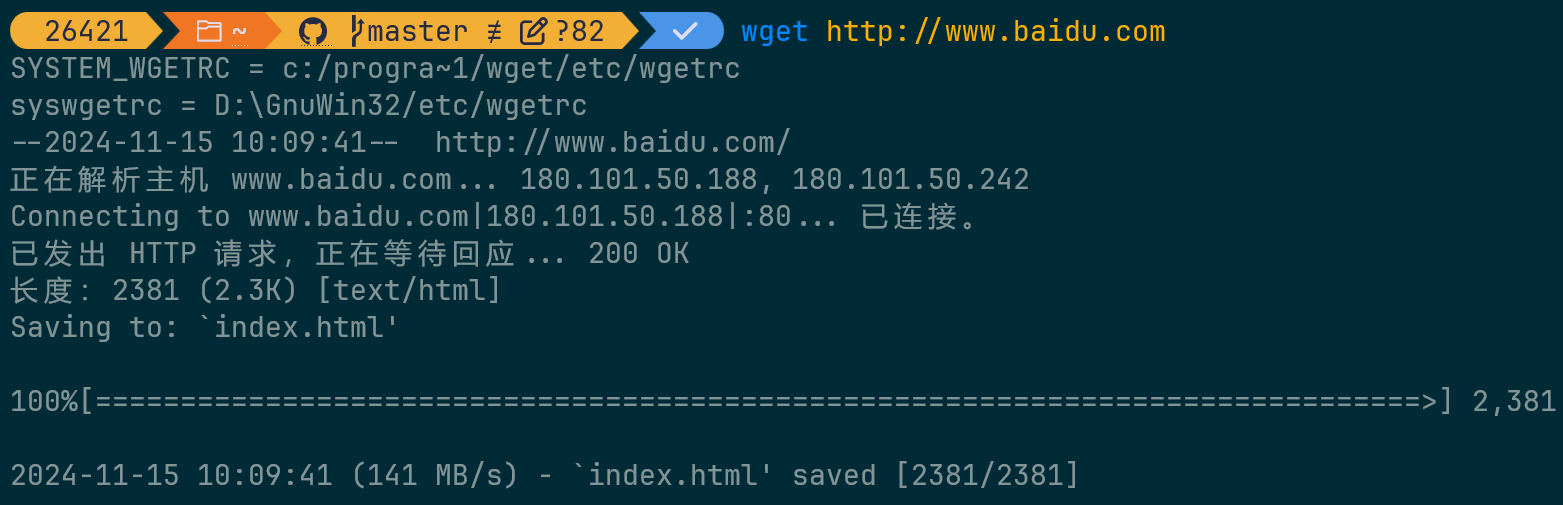
\includegraphics[width=0.4\textwidth]{lab1/WgetResult.png}
  \caption{Wget Result}
\end{figure}

\subsection{启动 Wireshark 捕获数据包}

启动 Wireshark,按照实验要求将捕获选项设置为:已连接的以太网,设置捕获过滤器为 tcp port 80,将混杂模式设为关闭,勾选 enable network name resolution。

\begin{figure}[H]
  \centering
  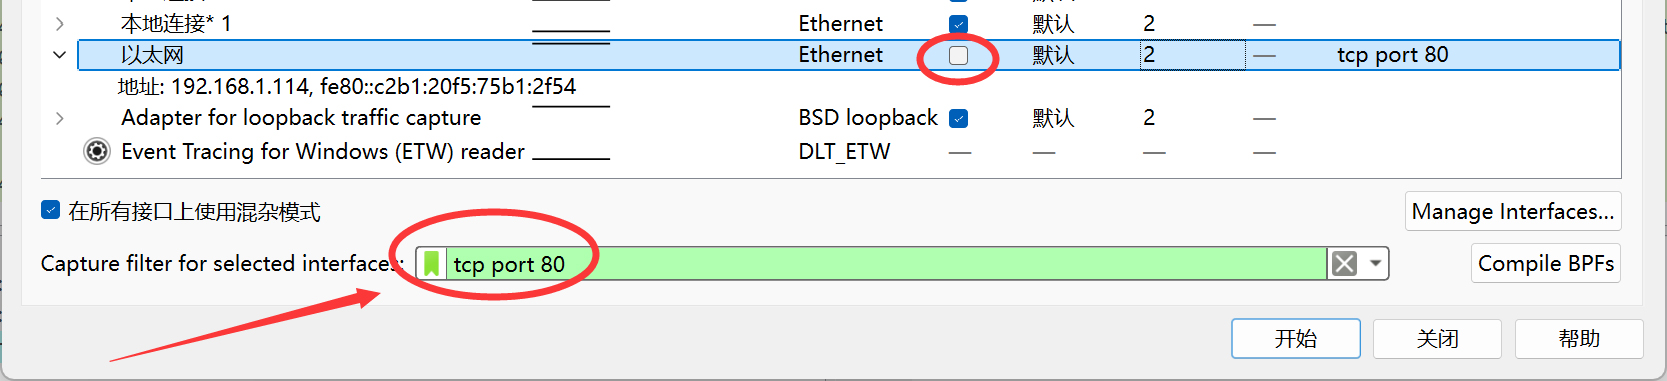
\includegraphics[width=0.6\textwidth]{lab1/fitler.jpg}
  \caption{Wireshark Filter}
\end{figure}

设置 rename 选项为开启:

\begin{figure}[H]
  \centering
  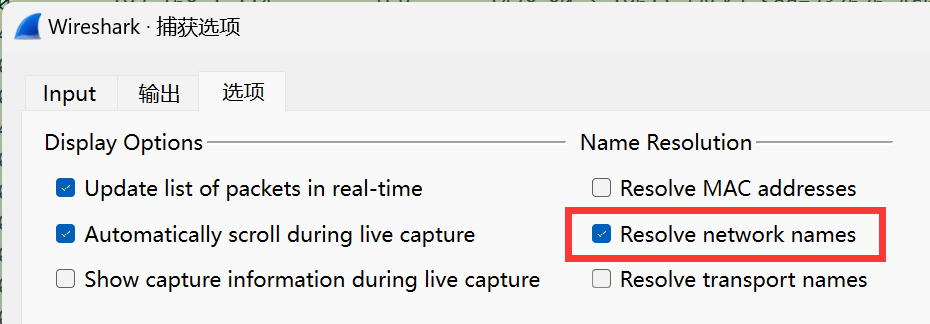
\includegraphics[width=0.4\textwidth]{lab1/rename.png}
  \caption{Wireshark Rename}
\end{figure}

\subsection{通过 Wireshark 捕获数据包}

在命令行中输入命令\texttt{wget http://www.baidu.com},等待回应。

\begin{figure}[H]
  \centering
  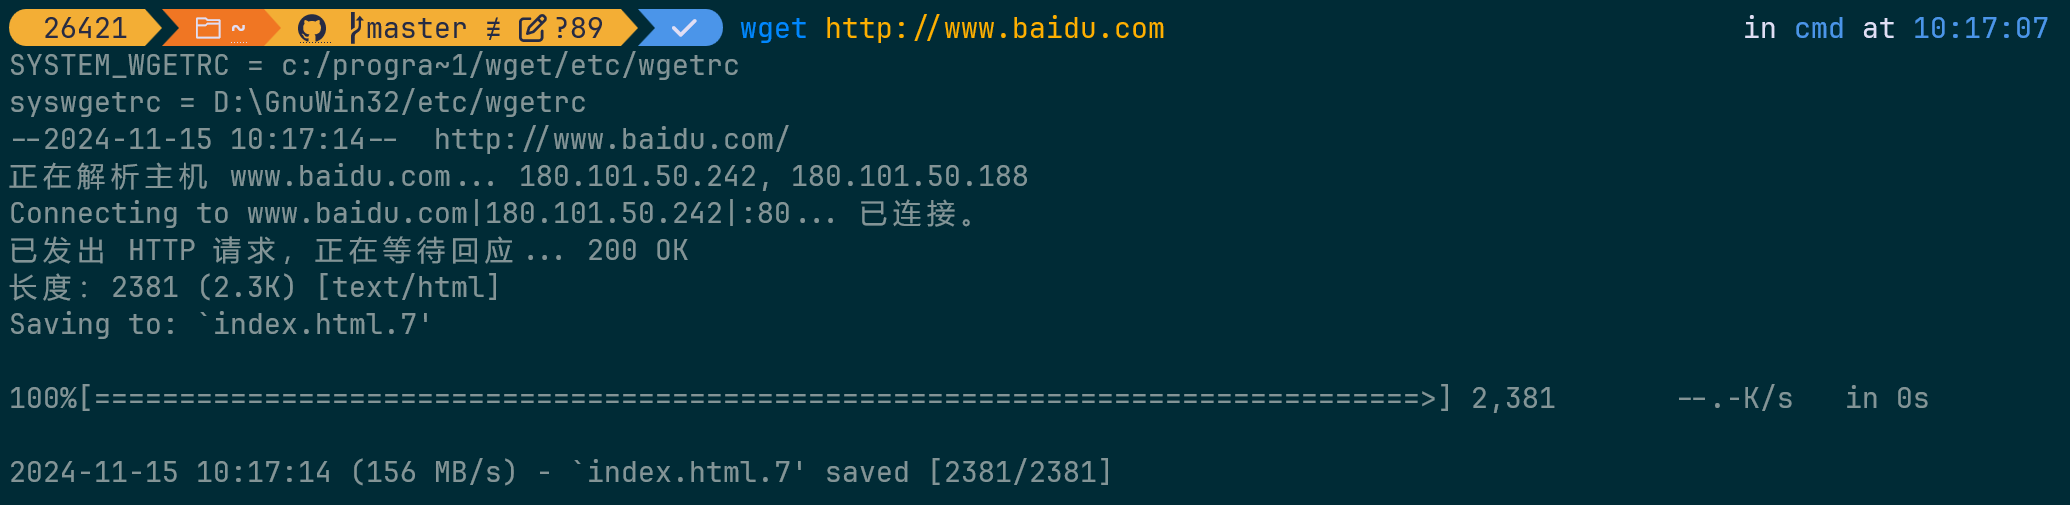
\includegraphics[width=0.6\textwidth]{lab1/againwget.png}
  \caption{Again Wget}
\end{figure}

在 Wireshark 捕获数据包,停止捕获。

\begin{figure}[H]
  \centering
  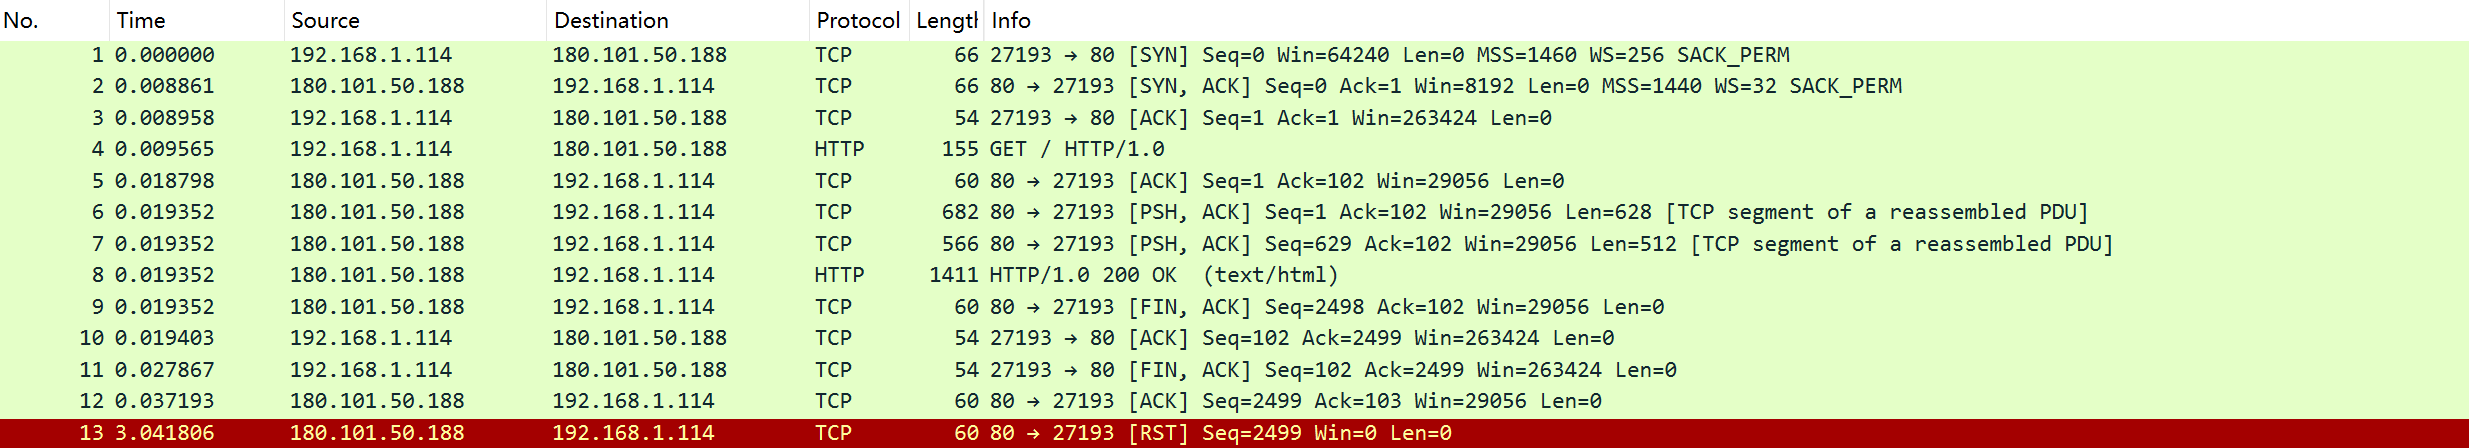
\includegraphics[width=0.8\textwidth]{lab1/httpget.png}
  \caption{HTTP Get}
\end{figure}


根据 TCP 三次握手的内容,即:三次握手过程总结

\begin{itemize}
  \item 第一次握手(SYN):客户端发送 SYN 报文,表示请求连接。
  \item 第二次握手(SYN-ACK):服务器收到 SYN 报文后,返回 SYN-ACK 报文,表示同意连接并同步序列号。
  \item 第三次握手(ACK):客户端收到 SYN-ACK 报文后,发送 ACK 报文,确认连接建立。
\end{itemize}

\textbf{具体而言,抓包获取的内容如下}:

\begin{itemize}
  \item wget 输出显示请求了 http://www.baidu.com,服务器 IP 地址为 180.101.50.188,该 IP 与抓包中相关帧中的 IP 匹配。
  \item 抓包的第 1 帧表示 TCP 三次握手的初始 SYN 包,第 2-3 帧完成握手的 SYN-ACK 和 ACK。
  \item 第 4 帧显示客户端(192.168.1.114)向服务器(180.101.50.188)发送的 HTTP GET 请求 (GET / HTTP/1.0)。
  \item 第 8 帧显示服务器返回 HTTP 200 OK 响应,表明内容已成功接收。此响应包含 HTTP 数据,共 1411 字节。
  \item 第 9-12 帧为客户端和服务器之间的连接关闭过程,其中 9 和 11 帧为 FIN 包,10 和 12 帧为 ACK 包,最后第 13 帧为服务器发出的 RST 包。
\end{itemize}

\subsection{分析协议包}

选中 HTTP 协议中 含有 GET 的协议包,再查看带有 200 OK 字样的返回包,查看其内容:

\begin{figure}[H]
  \centering
  \begin{subfigure}{0.8\textwidth}
    \centering
    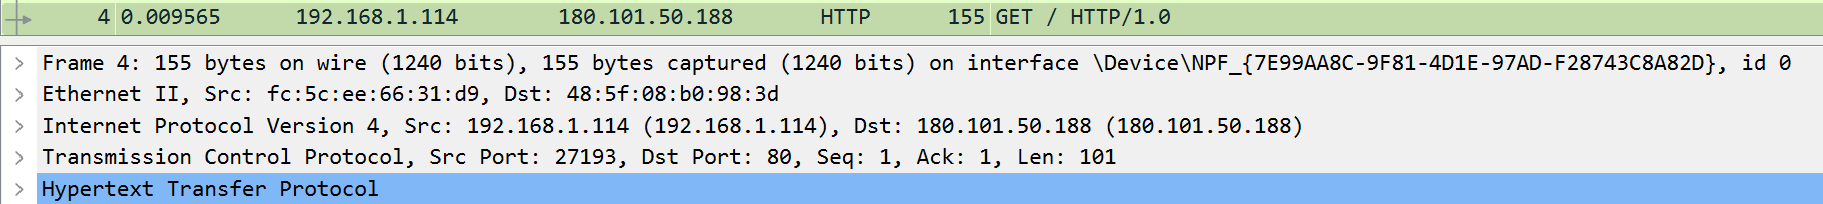
\includegraphics[width=\textwidth]{lab1/getcontent.png}
    \caption{HTTP GET}
  \end{subfigure}
  
  \begin{subfigure}{0.8\textwidth}
    \centering
    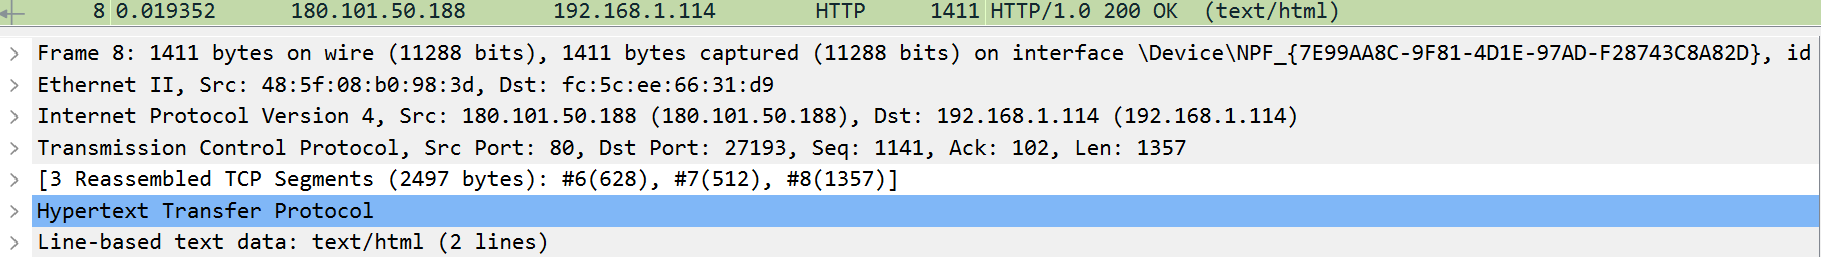
\includegraphics[width=\textwidth]{lab1/getcontentok.png}
    \caption{HTTP GET 200 OK}
  \end{subfigure}
\end{figure}

进入下方含有十六进制码的区域,按照实验手册中所描述的协议包结构进行分析。
Frame 字段是总体信息的记录,Ethernet 字段是以太网信息的记录,IP 字段是 IP 信息的记录,TCP 字段是 TCP 信息的记录,HTTP 字段是 HTTP 信息的记录。
通过点击不同的字段,可以总结为下图所示的结构:

\begin{figure}[H]
  \centering
  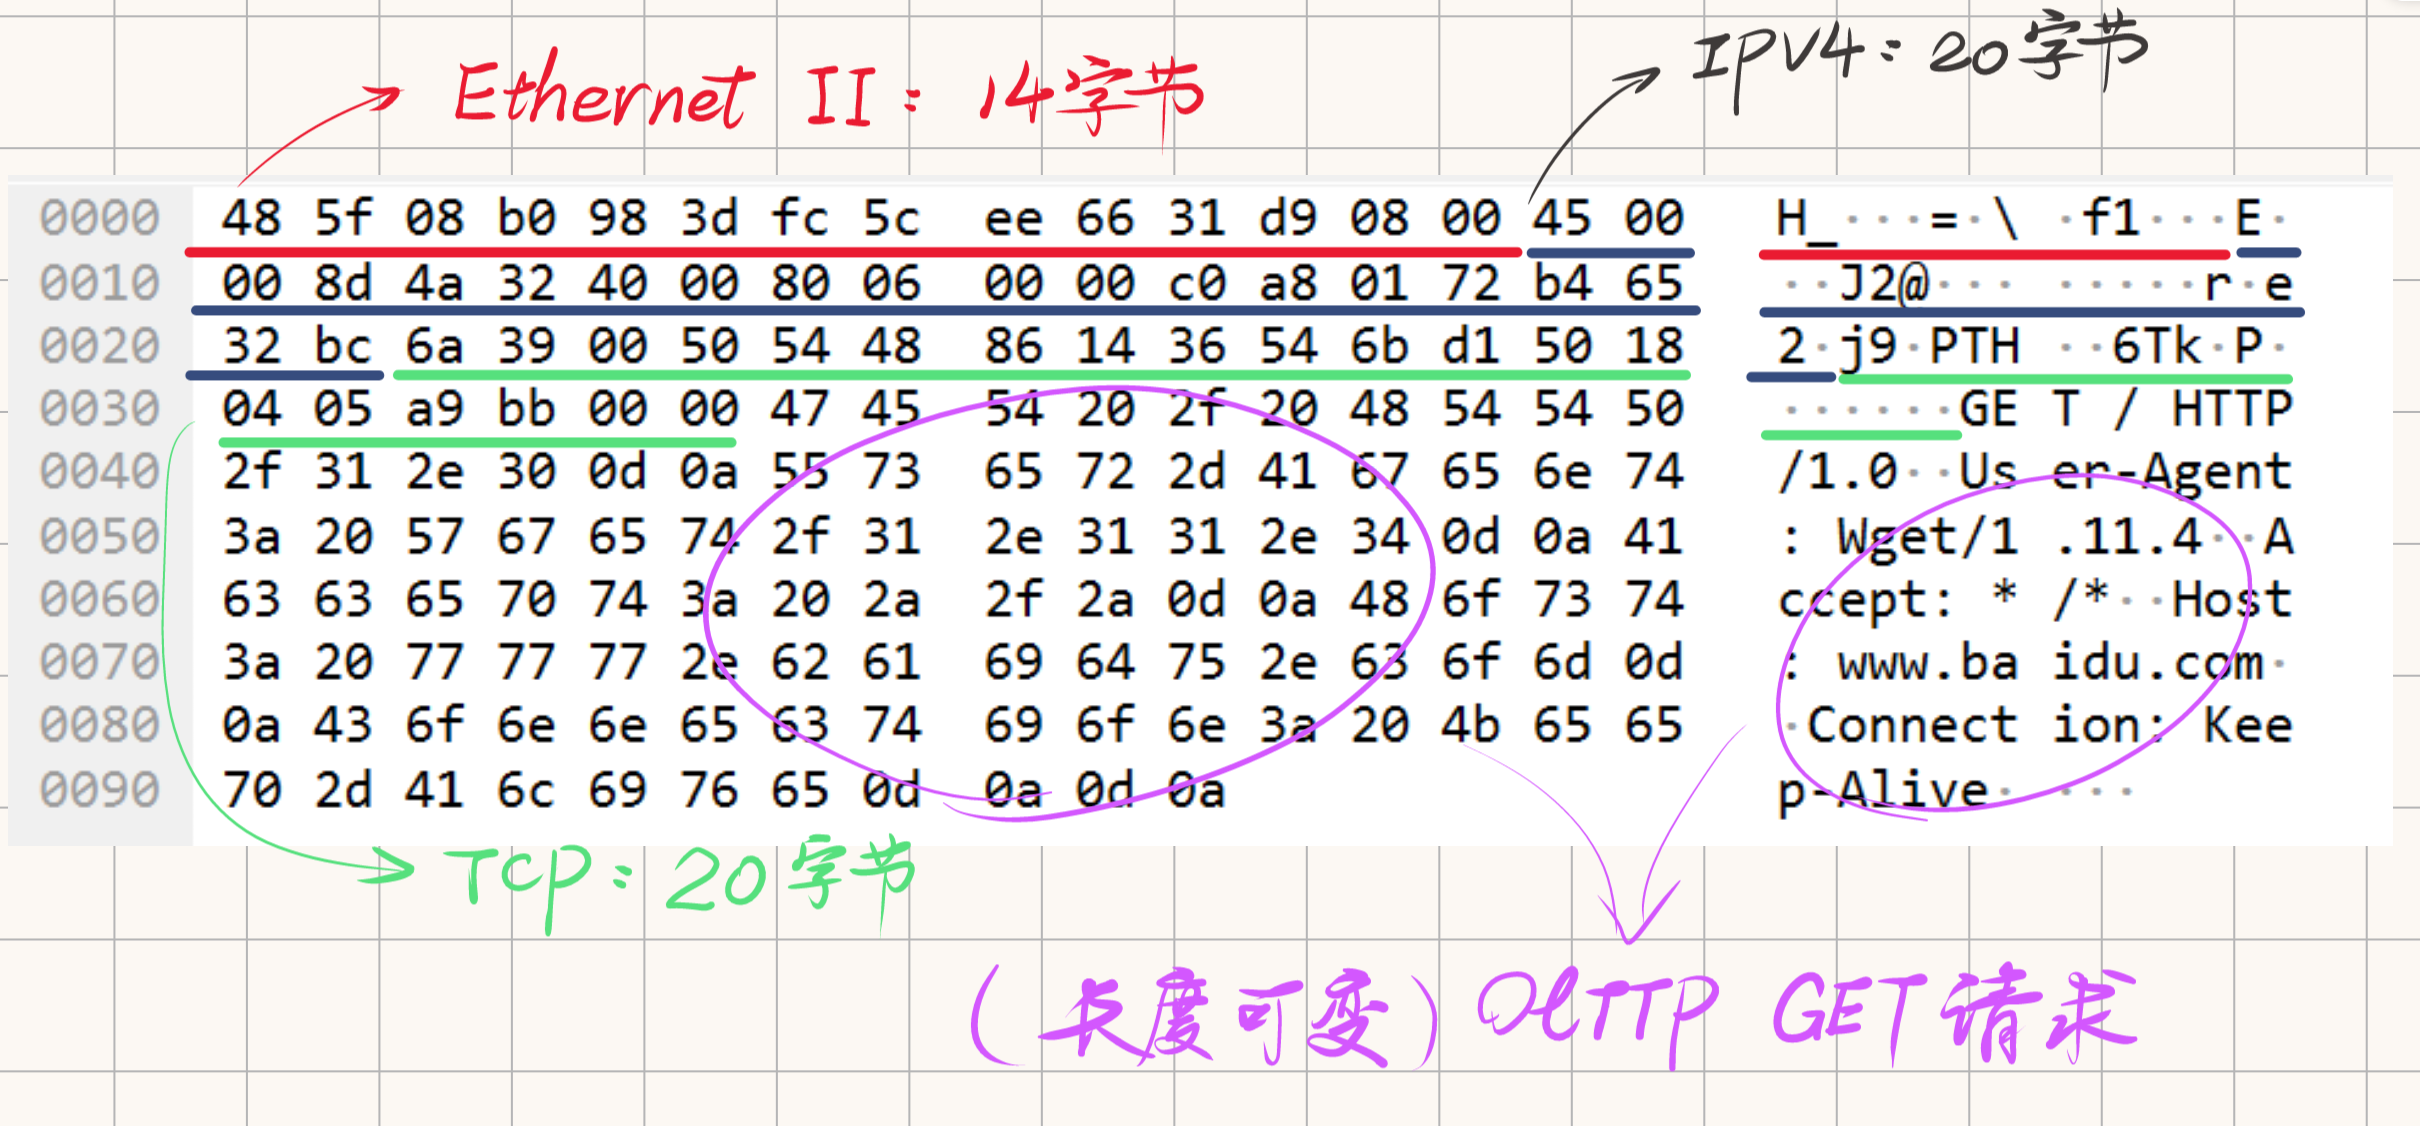
\includegraphics[width=0.55\textwidth]{lab1/structureanalysis.png}
\end{figure}

按照实验手册所要求的画为长条状的矩形,可为下图的结构:

\begin{figure}[H]
  \centering
  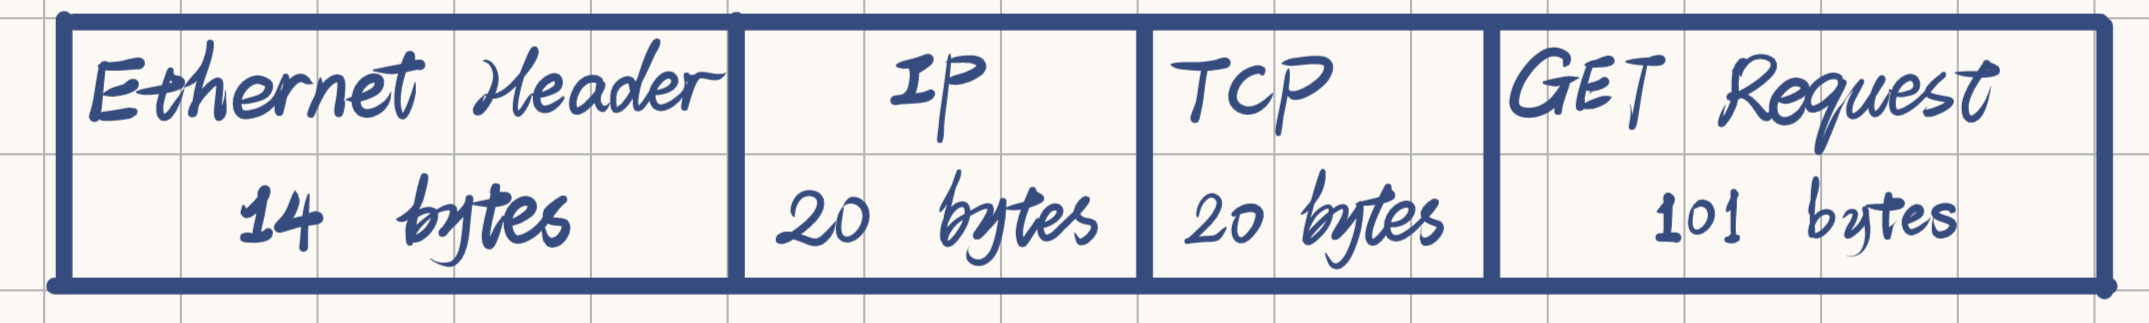
\includegraphics[width=0.5\textwidth]{lab1/structure.png}
\end{figure}

\subsection{分析协议开销}

将HTTP数据(报头和消息)视为网络携带的有用数据,而将较低层报头(TCP、IP和以太网)视为开销。

\begin{figure}[H]
  \centering
  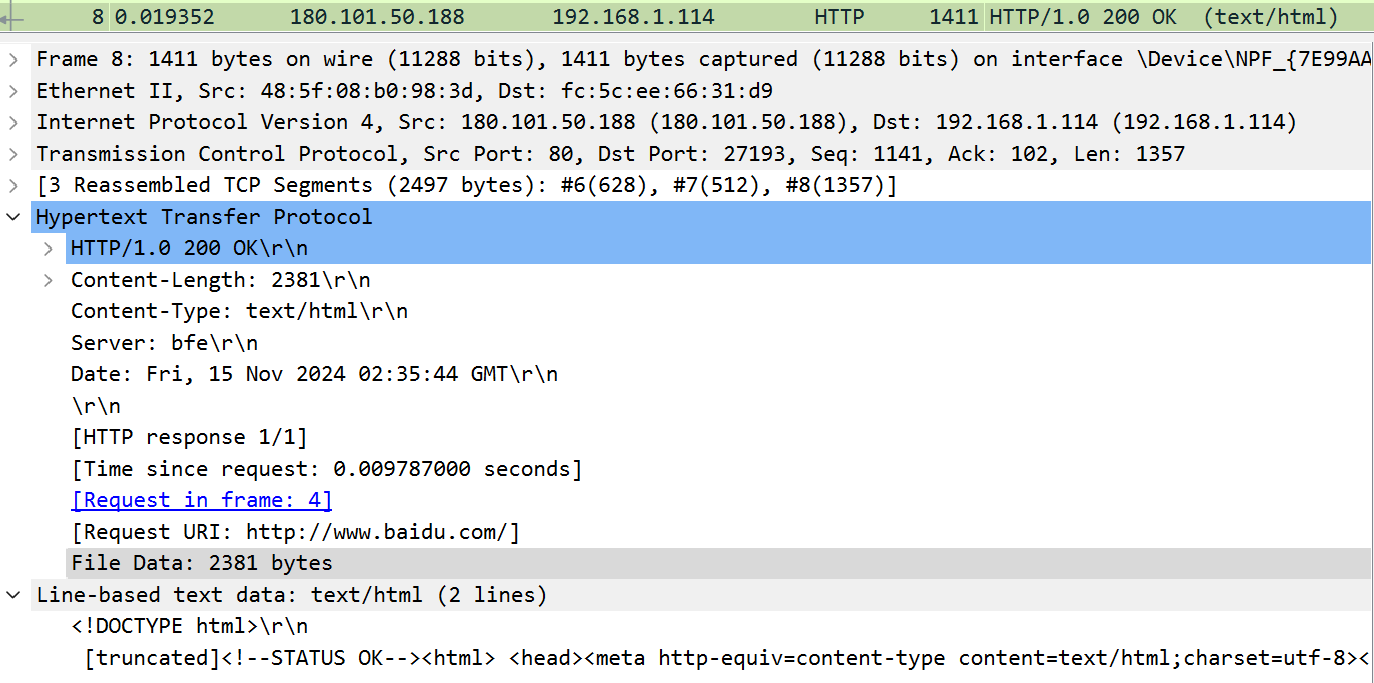
\includegraphics[width=0.55\textwidth]{lab1/cost.png}
  \caption{Protocol Overhead}
\end{figure}

展开 HTTP GET 200 OK 可见,真正传输的 File Data 作为有效数据实际的 HTTP 内容负载,在此应为 2381 字节。

下面,我观察到 HTTP 相应数据分成了 3 个 TCP 包发送,三个重新组装的 TCP 段:

\begin{center}
Frame 6(628 字节)、Frame 7(512 字节)和 Frame 8(1357 字节)
\end{center}

它们组成了一个完整的 HTTP 响应,共 2497 字节,经过重新组装形成完整的 HTTP 数据。

\begin{figure}[H]
  \centering
  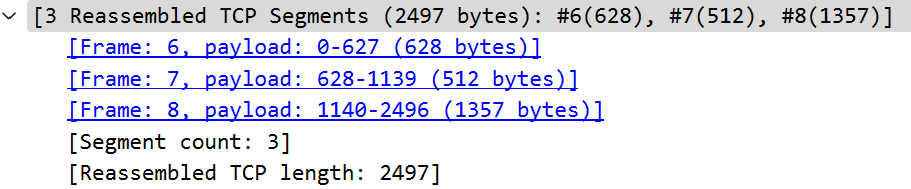
\includegraphics[width=0.55\textwidth]{lab1/tcps.png}
  \caption{Multi TCP Packets}
\end{figure}

\begin{ans}{Cost}{Cost}
此时,分成 3 个 TCP 包发送会造成协议开销,按照上面所分析的过程,可以知道协议开销应该是:

\[
3 \times [14(\text{Ethernet}) + 20(\text{IP}) + 20(\text{TCP})] = 162 Bytes.
\]

故协议开销占总体数据传输的占比应为:

\[
\frac{162}{162 + 2381} \times 100 \% \approx 6.37\%. 
\]
\end{ans}

\subsection{分析解复用键}

IP必须能够确定IP消息的内容是TCP数据包,以便将其交给TCP协议进行处理。答案是,协议使用其报头中的信息(称为“解复用密钥”)来确定更高层。

回顾题目的问题,如下所示:

\begin{itemize}
  \item 1.以太网头部中哪一部分是解复用键并且告知它的下一个高层指的是IP,在这一包内哪一个值可以表示IP?
  \item 2.IP头部中哪一部分是解复用键并且告知它的下一一个高层指的是TCP,在这一包内哪一个值可以表示TCP?
\end{itemize}

回顾抓包内容:

\begin{figure}[H]
  \centering
  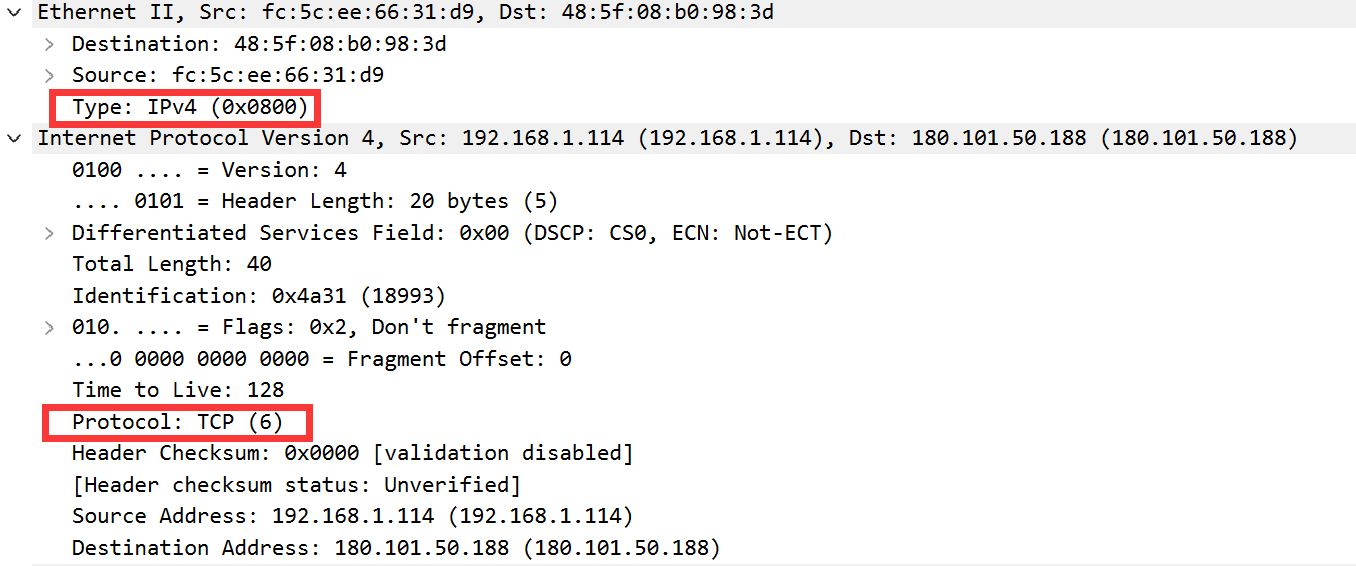
\includegraphics[width=0.6\textwidth]{lab1/demultiplexing.png}
  \caption{解复用键抓包分析}
\end{figure}

Type: IPv4(0x0800)是解复用键并且告知它的下一个高层是IP。
其中,0x0800表示IP。

\begin{figure}[H]
  \centering
  \begin{subfigure}{0.6\textwidth}
    \centering
    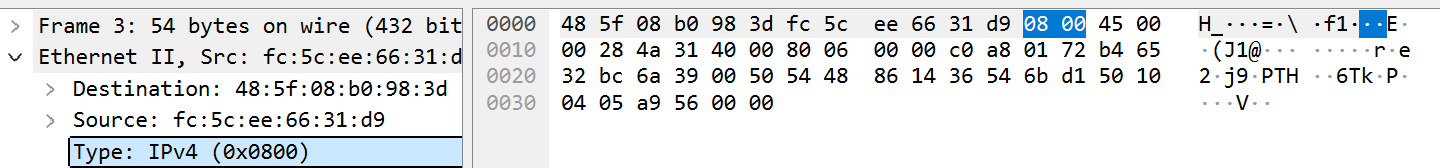
\includegraphics[width=\textwidth]{lab1/IPV4.png}
    \caption{IPv4 Demultiplexing}
  \end{subfigure}
  
  \bigskip

  \begin{subfigure}{0.5\textwidth}
    \centering
    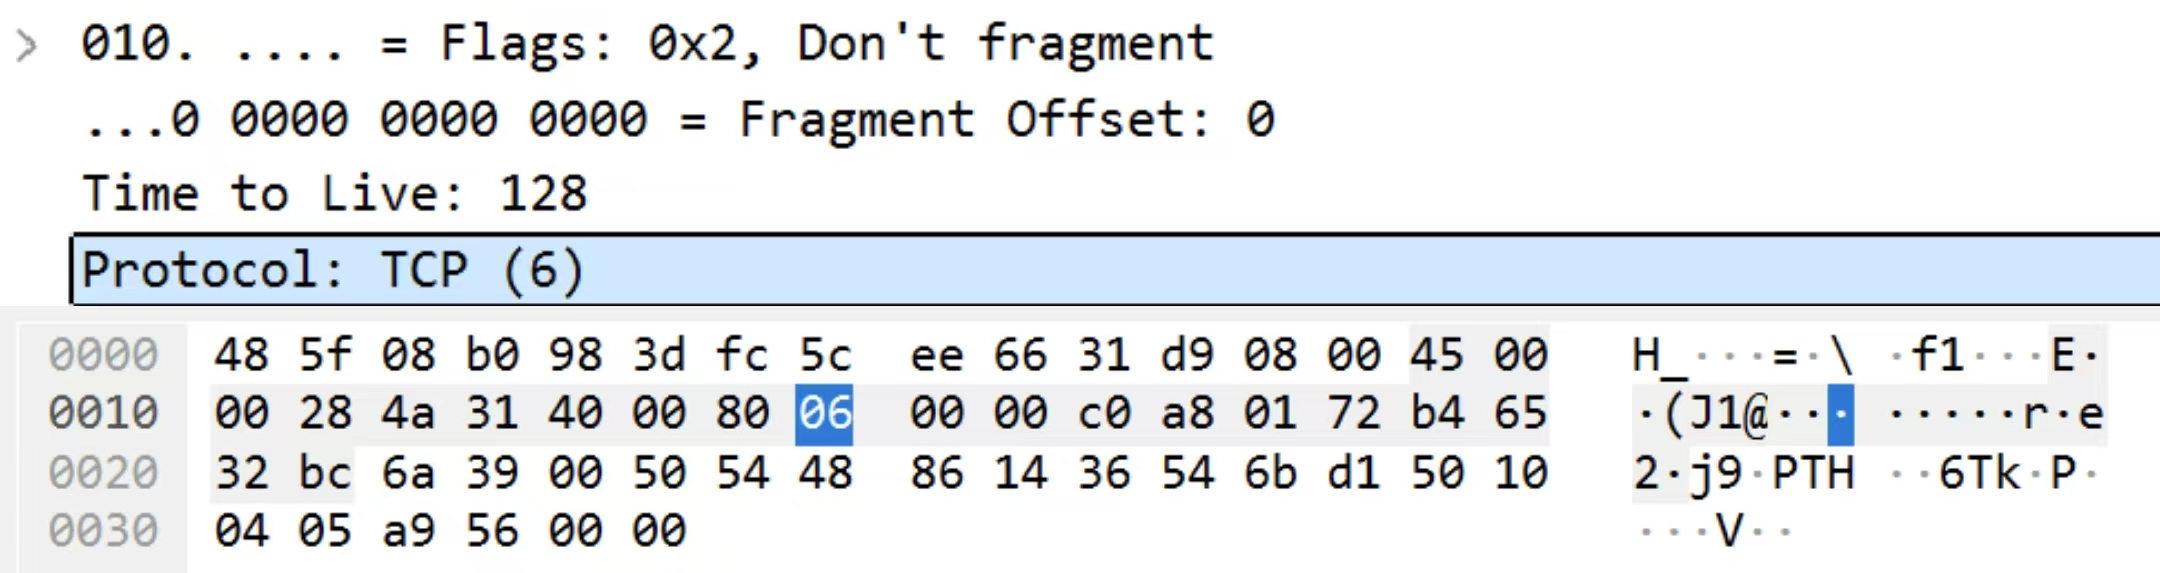
\includegraphics[width=\textwidth]{lab1/demul.jpg}
    \caption{TCP Demultiplexing}
  \end{subfigure}
\end{figure}

Protocol: TCP (6)是解复用键并且告知它的下一个高层指的是TCP。
其中,6表示TCP。

\subsection{课后思考题}

\subsubsection{Question 1}
Look at a short TCP packet that carries no higher-layer data. To what entity is this packet destined?

观察一个携带无更高层数据的短 TCP 包。该包的目的实体是什么?

\subsubsection*{解答}

一个携带无更高层数据的短 TCP 包通常用于连接管理和控制,而不是数据传输。这种包的示例包括:

SYN 和 ACK 包,用于建立连接的三次握手过程。
FIN 和 RST 包,用于终止连接。
空的 ACK 包,用于确认数据包的接收,而无需返回任何数据。
这些包被发送到目标设备的 TCP 层,并用于管理连接状态,而不是被转发到更高层的协议(如 HTTP),因为它们不携带更高层的有效负载。

\subsubsection{Question 2}

How would the drawings differ between the first and last TCP packet carrying the web response?

携带网页响应的第一个和最后一个 TCP 包在绘图上有何不同?

\subsubsection*{解答}

在携带网页响应的第一个 TCP 包中,包含 HTTP 响应头的开始部分,包括状态码以及响应数据的初始部分。

而在携带网页响应的最后一个 TCP 包中,会包含 HTTP 负载的结尾部分。

主要区别在于每个包所承载的 HTTP 负载部分,只有第一帧具有 HTTP 协议头,而最后一个包携带消息的结尾,有效载荷。
两个包都包含 TCP 头,但序列号和负载内容反映了它们在 HTTP 消息中的不同位置。

\subsubsection{Question 3}
How would the model change if a lower layer adds encryption?

如果低层添加加密,模型将如何改变?

\subsubsection*{解答}

如果低层添加加密,从更高层传递下来的数据(如 HTTP 消息)将在低层(通常是传输层如 TLS 或网络层如 IPsec)被加密。

原始的更高层消息被转变成一个加密的负载,随后由低层添加头部。
只有拥有解密密钥的实体(如客户端和服务器)才能访问原始消息。
这种模型通常称为“加密封装”,因为数据被封装在额外的加密层中,以保护消息在网络中的传输安全。

\subsubsection{Question 4}
How would the model change if a lower layer adds compression?

如果低层添加压缩,模型将如何改变?

\subsubsection*{解答}

如果低层添加压缩,从更高层传递下来的数据在被低层添加头部之前被压缩。这会在以下方面改变模型:

数据被低层压缩成较小的格式。
随后低层会在压缩后的数据上添加自己的头部。
接收端需要在将消息传递到更高层之前解压缩负载。
这种压缩封装使得数据传输更高效,因为压缩减少了数据大小,但接收端必须在将消息传递给更高层之前对其进行解压缩。

\section{实验结果总结}

在本次实验中,我通过 Wireshark 软件学会了对 HTTP 协议进行抓包分析,验证了协议分层模型在实际传输中的应用,
并深入了解了每一层协议的报文结构和协议开销。

\begin{itemize}
  \item 使用 Wget 获取了 http://www.baidu.com 的网页内容,并通过 Wireshark 观察到 HTTP 请求和响应的传输过程。
  \item 使用 Wireshark 进行抓包分析,获取到了 TCP 三次握手、HTTP GET 请求、HTTP 响应以及 TCP 连接终止的完整过程。
  \item 计算了 HTTP 传输的协议开销,验证了在数据分片传输的情况下,各层协议头部会增加协议开销。
  \item 见识了了解了复用键在以太网、IP 和 TCP 层的重要性,并观察到如何通过解复用键确定上层协议。
\end{itemize}

\section{附录}

\subsection*{参考资料}

\begin{itemize}
  \item \href{https://wenku.csdn.net/answer/ca032a216e634b30890de2bea74f3924}{\underline{怎么用wireshark看数据包的开销}}
  \item \href{https://blog.csdn.net/bigbangbangbang1/article/details/142208991}{\underline{这么详细的Wireshark的抓包和分析,工作中是没人告诉你的!}}
\end{itemize}
\end{document}